\chapter{Návrh riešenia}

\section{Meranie hĺbky pamäte samorganizujúcich sa máp}

\subsection{Trénovacie dáta}
Vstupné sekvencie teda pozostávajú zo sekvencie písmen anglickej abecedy (26 písmen).
Čo budú mať tieto trénovacie množiny spoločné je, že sú tvorené/generované určitým nenáhodným spôsobom 
a teda môžeme na nich natrénovať rekurentné neurónové siete. Inými slovami dokážu v nich 
neurónové siete zachytiť nejakú vnútornú reprezentáciu.
Samotné vstupy (trénovacie príklady) pre sieť budú zakódované jednotlivé písmená z trénovacej sekvencie.
Písmená kódujem do 26 prvkového vektora, ktorého prvky budú nuly a jednotka (pre každé písmeno na unikátnej pozícii).

\subsection{Spôsob uchovávania informácii s SOM}
Každý neurón bude mať množinu, v ktorej si bude pamätať pre aký vstup bol víťazom. 
Nebude si však ukladať iba aktuálny vstup (aktuálne písmeno), 
ale $k$ posledných písmen z trénovacej množiny - posuvné okno (ang. sliding window). 

Z týchto dát si viem potom ďalej vytvoriť hitmapu, ktorá mi bude vizualizovať, na aké vstupy neuróny reagovali.

\begin{figure}[H]
	\centering
	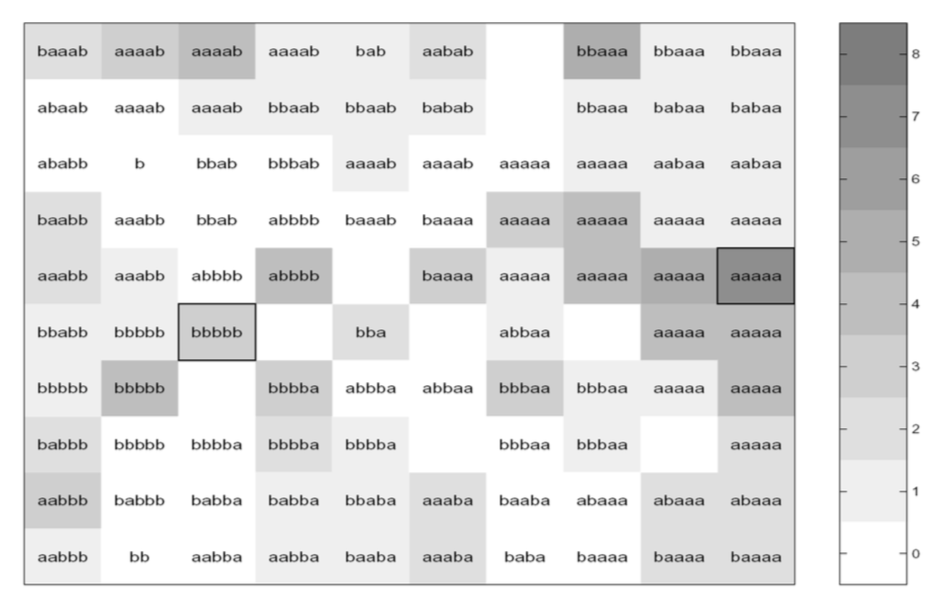
\includegraphics[width=10cm]{assets/receptive_field}
	\caption{Hitmapa}
\end{figure}

Mierou hĺbky pamäte mapy bude potom vážený priemer dĺžky najdlhších spoločných podpostupností písmen v množinách jednotlivých neurónov. Dĺžku najdlhšej podpostupnosti budem určovať od konca sekvencií v množine. Priemer pamäťových hĺbok jednotlivých neurónov musí byť vážený, aby neuróny, %s väčším počtom víťazov mali vyššiu váhu ako neuróny s menším počtom víťazov.
ktoré zvíťazili pre viac vstupov, mali vyššiu váhu ako víťazné neuróny pre menší počet vstupov.
Po každej trénovacej epoche (prechode trénovacou množinou) budem vedieť určiť pamäťovú hĺbku mapy.
Vďaka tomu, že neuróny rekurentných sietí majú okrem normálnych váh aj kontextové váhy, ktoré uchovávajú informáciu z predchádzajúceho kroku,  môže sa stať, že rovnaké písmeno zo vstupu bude mať rôzne víťazné neuróny počas trénovania.

Samotná pamäťová hĺbka je relatívna a závisí od veľkosti posuvného okna.
Veľkosť posuvného okna má zmysel zvyšovať iba pokiaľ nám stúpa pamäťová hĺbka, inými
slovami toto okno musí byť minimálne tak veľké ako je pamäťová hĺbka siete.

Počet neurónov v mape volíme podľa množstva rôznych slov v použitej trénovacej
množine.

Tradeoff medzi rozlišovaciou schopnosťou jednotlivých slov a schopnosťou
zachovať podobné slová topologicky čo najbližšie pri sebe.

Na trénovanie a vyhodnocovanie pamäťovej hĺbky som si vytvoril 3 sady 
trénovacích príkladov. 
Prvá sada sú najednoduchšie sekvenice (slová), ktoré obsahujú veľké množstvo regularít a malé množstvo rôznych písmen.
Napríklad sekvencie ako $aaabbb$,  $bbbaaaaa$.
Druhou sadou budú slová generované Reberovým automatom.
Treťou sadou trénovacích príkladov budú najzložitejšie sekvencie, resp. slová z určitého korpusu. 
Túto sadu budem používať ako performance benchmark. 

\section{mSOM s leaky integration contextom}
Pre potreby testovania pamäťovej hĺbky sme si vytvorili modifikovanú verziu mSOM, ktorá používa iný kontext.
V pôvodnej mSOM bol kontext tvorený lineárnou kombináciou vlastností víťazného neurónu z predchádzajúceho kroku.
V našej modifikovanej verzii mSOM budú kontext tvoriť samotné vstupné vektory z predchádzajúcich krokov.

Všetko ostatné zostane rovnaké ako v pôvodnej mSOM.
Samotný kontext budem počítať pomocou nasledujúceho rekurzívneho vzťahu:
\begin{equation}
	c = \beta^{0} \cdot x_{t} + \beta^{1} \cdot x_{t-1} + 
	\beta^{2} \cdot x_{t-2}....
\end{equation}

$\beta$ parameter je číslo $\beta < 1 \ve$

Tým zabezpečím, že kontext bude tvorený lineárnou kombináciou 
predchádzajúcich vstupov a čím ďalej idem do minulosti, tým majú tieto vstupy 
menšiu váhu (vďaka umocňovaniu beta parametra). Preto sme túto modifikovanú mSOM nazvali 
mSOM s miznúcim kontextom (vanishing mSom).

\section{Hľadanie ideálnych (hyper) parametrov}
Ako prvý parameter potrebujem zoptimalizovať veľkosť posuvného okna, tak aby bol väčší ako
maximálna pamäťová hĺbka. Toto docielim jednoducho tým, že ho dám rozumne veľký, resp. v prípade
potreby ho budem zvyšovať.

Ďaľšie dôležité parametre, ktoré potrebujem optimalizovať sú $alpha$ a $beta$ parametre, ktoré 
sa používajú pri počítaní vzdialenosti a určujú akú váhu má aktuálny vstup a akú váhu má kontext.
Toto neviem spraviť nijak inak, iba postupním skúšaním rôznych kombinácii týchto parametrov. 
$alpha$ aj $beta$.

Optimálne $alpha$ a $beta$ parametre, ktoré dávajú najlepšie výsledky som hľadal nasledujúcim
spôsobom:

Naprogramoval som si skript, pomocou ktorého trénujem sieť s rôznymi parametrami.
Výsledky som si počas trénovania zaznamenával.
Následne som si vykreslil 3D grafy pre každý typ trénovanej siete (msom, recsom, vmsom), 
kde na x-ovej osy sú hodnoty alpha parametra, na y-ovej osy sú hodnoty beta parametra a
na z-ovej osy sú hodnoty pamäťových hĺbok.
Na začiatok som zvyšoval parametre po hodnote $0.1$.

% TODO ukazky grafov parametrov pre jednotlive siete







